
\section{Pull-back Prior}\label{sec:pull_back_prior}

\subsection{Intuition of Pull-back Prior}\label{subsec:intuition}

The formula of Pull-back Prior is given by:
\begin{equation}\label{eq:pull_back_prior}
	p_\lambda(z) = \frac{1}{Z} p_\mathcal{N}(z) \cdot e^{- \beta D(G(z))} \tag{4}
\end{equation}
where $p_\mathcal{N}$ is a simple prior, $D$ is a discriminator, $G$ is the generator $G(z) = \E_{p_\theta(x|z)} x$, $Z$ is the partition function $Z = \int_{\mathcal{Z}} p_\mathcal{N}(z) \exp\{- \beta * D(G(z))\} \dd z$ and $\beta$ is a learnable scalar.

An intuitive explanation of Pull-back Prior is given following: We would like to get a more powerful prior than simple prior $p_\mathcal{N}$. A simple way is to improve the density of $z$ which generates better data and decrease the density of $z$ which generates worse data. $D$ is a discriminator to assess the quality of $x$. When $D(x)$ is less, $x$ is more similar to real data and of higher quality, as shown in \cref{fig:interpolate}. We could pull-back the discriminator from data space to latent space, and function $D(G(z))$ represents the quality of the data generated by $z$. To improve and decrease the density at better $z$ and worse $z$, we modify $p_\mathcal{N}(z)$ by $\beta D(G(z))$ and then normalize it by $Z$, and finally we obtain the Pull-back Prior. 

We obtain the basic formula of Pull-back Prior, and $p_\mathcal{N}$ is a special case where $\beta = 0$. The theoretical derivation for Pull-back Prior is provided in \cref{subsec:inference}. However, it remains some troubles about how to obtain $D$ and $G$, determine $\beta$, and calculate $Z$. 

\begin{figure}[tb]
	\centering
	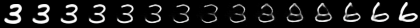
\includegraphics[width=0.9\columnwidth]{../figures/interpolate}
	\caption{
	The discriminators on above images (generated by linear interpolation of two sample from $q_\phi(z)$), are better at both sides and worse at mid, which validates the intuition that discriminator can assess the quality of images. Moreover, the density of $z$ which generate better images will increase, and the density of $z$ which generate worse images will decrease. 
%2825-plot_samples mean and std is 9.528099, 0.0050279954
%[array([[9.547822]], dtype=float32), array([[9.583102]], dtype=float32), array([[9.603901]], dtype=float32), array([[9.626318]], dtype=float32), array([[9.633714]], dtype=float32), array([[9.632847]], dtype=float32), array([[9.631333]], dtype=float32), array([[9.640044]], dtype=float32), array([[9.631817]], dtype=float32), array([[9.654361]], dtype=float32), array([[9.641564]], dtype=float32), array([[9.600273]], dtype=float32), array([[9.559095]], dtype=float32), array([[9.533435]], dtype=float32), array([[9.468535]], dtype=float32)]
%Normalized is [  3.92263684,  10.93934971,  15.07598834,  19.53442519,
%        21.00538915,  20.83295462,  20.53184058,  22.26434018,
%        20.62810161,  25.11179704,  22.56664754,  14.35442841,
%         6.16468344,   1.06125793, -11.84647066]
	}
	\label{fig:interpolate}
\end{figure}

\subsection{How to obtain $D$ and $G$}\label{subsec:determine_D_and_G}
By definition in \cref{eq:pull_back_prior}, $G$ is defined, and in practical networks, it is generated by neural network and $p_\theta(x|z)$ set it as mean (\EG $p_\theta(x|z)$ is Gaussian or Bernouli). 

$D$ plays an important role in Pull-back Prior. We propose two way to obtain $D$ and compare their difference detaily in \cref{subsec:improve_of_vaepp} and \cref{subsec:naive_vaepp}. 

\subsection{How to determine $\beta$}\label{subsec:determine_beta}

Theoretically, $\beta$ in \cref{eq:pull_back_prior} represents how far $p_\lambda$ is from $p_\mathcal{N}$, shown in \cref{subsec:inference}.
%but how to decide the value of $\beta$? When $\beta$ is smaller, the difference between $p_\lambda$ and $p_\mathcal{N}$ is less, \IE the influence of discriminator is severely limited. When $\beta$ is larger, $p_\lambda$ is farther from $p_\mathcal{N}$. Noticing that in \cref{eq:final_optimization}, we simplify the optimization of $D$ by an approximated $D$, if $p_\lambda$ is too far from $p_\mathcal{N}$, this approximation will become invalid. 
%Consequently, $\beta$ should be set to an appropriate value which can't severely limit the influence of discriminator and could ensure that approximated $D$ is valid. 
It is important to realize that the Pull-back Prior is serving for better ELBO. 
%Whatever the function family of $p_\lambda$ is limited or approximation $D$ is invalid, the ELBO will suffer. 
Therefore, it is reasonable to search $\beta$ by the optimization for ELBO ($\lambda$ contains $\beta$ and $\omega$, which is the parameters of $D$):
\begin{equation}
	\beta = \arg \min_{\beta} \mathcal{L}(\theta, \phi, \lambda) = \arg \min_{\beta} \mathcal{L}(\theta, \phi, \beta, \omega) \tag{5}
\end{equation}
The optimization process of $\beta$ depends on $\partial \mathcal{L}/\partial \beta$:
\begin{align*}\label{eq:behavior_of_beta}
\frac{\partial \ln Z}{\partial \beta} &= \frac{1}{Z} \int p_\mathcal{N}(z) e^{-\beta D(G(z))} \cdot (-D(G(z))) \dd z \\
&=  \E_{p_\lambda(z)} - D(G(z))  \\
\frac{\partial \mathcal{L}}{\partial \beta} &= \E_{q_\phi(z)}[ -D(G(z))] - \frac{\partial \ln Z}{\partial \beta} \\
&= - \E_{q_\phi(z)}[ D(G(z))] + \E_{p_\lambda(z)}[ D(G(z))]   \tag{6}
\end{align*}
The 1st term in \cref{eq:behavior_of_beta} is the mean of discriminator on data generated from $p_\lambda$. The 2nd term in \cref{eq:behavior_of_beta} is the mean of discriminator on reconstructed data which is nearly same as real data when reconstruction is well-trained. Hence, $\partial \mathcal{L}/\partial \beta = 0$ represents that the discriminator can't distinguish the reconstructed data (nearly same as real data) and generated data. It coincides the philosophy of GAN.

\subsection{The lower bound of $Z$}\label{subsec:determine_z}

The extract calculation of partition function $Z$ is difficult. But in VAE domain, it is acceptable to obtain a lower-bound of log-likelihood. Therefore, we propose a feasible evaluation for upper-bound of $Z$, called $\hat{Z}$, which will not over-estimate log-likelihood. 
It is given by:
\begin{align*}\label{eq:Z_estimator}
	Z = \E_{q_\phi(z)}\frac{f_\lambda(z)}{q_\phi(z)} \leq \E_{q_\phi(z)} \frac{f_\lambda(z)}{\hat{q}_\phi(z)} = \hat{Z} \tag{8}
\end{align*}
where $f_\lambda(z) = p_\mathcal{N}(z) \exp\{- \beta D(G(z))\}$ and $\hat{q}_\phi(z)$ is a lower-bound of $q_\phi(z)$. It is easy to show that
\begin{align*}
	p_\theta(x) = \int \frac{1}{Z} p_\theta(x|z) f_\lambda(z) \dd z &\geq \int \frac{1}{\hat{Z}} p_\theta(x|z) f_\lambda(z) \dd z \\
\mathcal{K} = \E_{q_\phi(z)} \frac{1}{Z} \ln f_\lambda(z) &\geq \E_{q_\phi(z)} \frac{1}{\hat{Z}}\ln f_\lambda(z) = \mathcal{\hat{K}} \\
\mathcal{L} = \mathcal{I} + \mathcal{J} + \mathcal{K} &\geq \mathcal{I} + \mathcal{J} + \mathcal{\hat{K}} = \mathcal{\hat{L}}
\end{align*}
Above ineqaulities show that, if we replace $Z$ by $\hat{Z}$ we will obtain lower-bound of log-likelihood and ELBO. Such that $\hat{Z}$ could be used in training and evaluation, and it will not over-estimate log-likelihood and ELBO. 

The key of \cref{eq:Z_estimator} is the choice of $\hat{q}_\phi(z)$. As we mentioned before, $q_\phi(z)$ is intractable to compute the exact density, but $q_\phi(z|x)$ is feasible. We introduce a lower-bound of  $q_\phi(z)$:
\begin{equation*}
	q_\phi(z) = \E_{p^*(x)} q_\phi(z|x) \approx \frac{1}{N}\sum_{i=1}^N q_\phi(z|x^{(i)}) \geq \frac{1}{N} q_\phi(z|x^{(j)})
\end{equation*}
where $x^{(j)}$ is a real data, $N$ is the size of training set and RHS is the $\hat{q}_\phi(z)$. To reduce the gap between $\hat{q}_\phi(z)$ and $q_\phi(z)$, $q_\phi(z|x^{(j)})$ should be one of the largest in summation. Therefore, we firstly sample $x^{(j)}$ form dataset, and then sample $z$ from $q_\phi(z|x^{(j)})$. By this way, $q_\phi(z|x^{(j)})$ is  large enough. 

In MNIST and other Bernouli image datasets, the number of Bernouli images sampled from real images might be numerous and $\hat{q}_\phi(z)$ might be underestimiated. To solve this it, we propose ELBO based on $q_\phi(z|e)$ instead of $q_\phi(z|x)$:
\begin{align*}~\label{eq:another_elbo}
	&\E_{p^*(x)} \ln p_\theta(x) \geq \E_{p^*(e)} \E_{p^*(x|e)} \ln \E_{q_\phi(z|e)} \frac{p_\theta(x|z)p_\theta(z)}{q_\phi(z|e)} \\
	 &= \E_{p^*(e)} \E_{p^*(x|e)} \E_{q_\phi(z|e)} \ln \frac{p_\theta(x|z)p_\theta(z)}{q_\phi(z|e)} \tag{7} \\
	 &= \E_{p^*(x)} \ln p^*(x) - \E_{p^*(e)} \E_{p^*(x|e)} KL(q_\phi(z|e), p_\theta(z|x))
\end{align*} 
where $p^*(x)$ is sampled from $p^*(e)$, and $p^*(x|e)$ means the sampling process from $e$. \cref{eq:another_elbo} is similar to the original ELBO~\cref{eq:ELBO}, and the above conclusion about learnable prior holds for \cref{eq:another_elbo} by repeating above inference. Moreover, the situation without Bernouli images is a special case where $p^*(x|e) = \delta(x - e)$. % Additionally, when $p_\theta(x|z)$ and $p^*(x|e)$ is both Bernouli, term $\E_{p^*(x|e)} \ln p_\theta(x|z)$ has analytical solution $x\log e+(1-x)\log(1-e)$, which could make the training and evaluation more stable (don't need sample $x$). 
Since $q_\phi(z|e)$ is known, $\hat{q}_\phi(z)$ is feasible by $\frac{1}{N} q_\phi(z|e^{(j)})$. 

By the theory of importance sampling, $p_\lambda$ is the optimal choice for the proposal distribution in estimation of $Z$ but it is expensive to sample from $p_\lambda$. 
\cite{bauer2019resampled} uses $p_\mathcal{N}$ as proposal distribution to estimate $Z$ but when $KL(p_\mathcal{N}, p_\lambda)$ is high, the variance of this estimation will be large. In experiment, $KL(q_\phi, p_\lambda)$ is much less than $KL(q_\phi, p_\mathcal{N})$ in trained model. Therefore, we choose $q_\phi(z)$ as proposal distribution and use a feasible $\hat{q}_\phi(z)$ to replace $q_\phi(z)$ in \cref{eq:Z_estimator}. The variance of $\hat{Z}$ is acceptable in experiment.  

In training, $\beta$ is trained from small to large and $KL(p_\mathcal{N}, p_\lambda)$ is so. Therefore, $p_\mathcal{N}$ is also used as proposal distribution in training. 